\chapter{Design}
\label{sec:design}

% Ist das zentrale Kapitel der Arbeit. Hier werden das Ziel sowie die
% eigenen Ideen, Wertungen, Entwurfsentscheidungen vorgebracht. Es kann
% sich lohnen, verschiedene Möglichkeiten durchzuspielen und dann
% explizit zu begründen, warum man sich für eine bestimmte entschieden
% hat. Dieses Kapitel sollte - zumindest in Stichworten - schon bei den
% ersten Festlegungen eines Entwurfs skizziert werden.
% Es wird sich aber in einer normal verlaufenden
% Arbeit dauernd etwas daran ändern. Das Kapitel darf nicht zu
% detailliert werden, sonst langweilt sich der Leser. Es ist sehr
% wichtig, das richtige Abstraktionsniveau zu finden. Beim Verfassen
% sollte man auf die Wiederverwendbarkeit des Textes achten.

% Plant man eine Veröffentlichung aus der Arbeit zu machen, können von
% diesem Kapitel Teile genommen werden. Das Kapitel wird in der Regel
% wohl mindestens 8 Seiten haben, mehr als 20 können ein Hinweis darauf
% sein, daß das Abstraktionsniveau verfehlt wurde.

%%%%%%%%%%%%%%%%%%%%%%%%%%%%%%%%%%%%%%%%%%%%%%%%%%%%%%%%%%%%%%%%%%%%%%%%%%%%%%%%
%                                                                              %
% MOTIVATION                                                                   %
%                                                                              %
%%%%%%%%%%%%%%%%%%%%%%%%%%%%%%%%%%%%%%%%%%%%%%%%%%%%%%%%%%%%%%%%%%%%%%%%%%%%%%%%
% Checked
\section{Motivation}


These days, complex simulation applications no longer fit on a single
computing device like a desktop computer. Therefore, parallel
computers are necessary instruments in scientific computing where time
to solution is important and a large amount of memory is required.  To
exploit the performance of a parallel computer, the application need
to be distributed onto the computing environment and exchange data by
communication over a network.

Assume, the mentioned parallel computer is a compute cluster
(Section~\ref{sec:cluster}). Furthermore assume, that cluster nodes
are equal among each other (\emph{vertical heterogeneous}) and a nodes
provide only one type of computing hardware (\emph{horizontal
  heterogeneous}). Usually, simulation applications are prepared for
this kind of vertical and horizontal heterogeneous clusters by domain
decomposition (Section~\ref{sec:domain_decomposition}). The simulation
domain is decomposed by a fixed algorithm into smaller chunks of work
called \emph{subdomains} and mapped onto the homogeneous network of
nodes. Subdomains exchange simulation specific data through predefined
paths among each other. This could mean inn concrete terms of MPI
(Section~\ref{sec:MPI}), every MPI process manages a subdomain and
communicates with a fixed set of other MPI processes by fixed
communication operations. The simulation algorithm and the
decomposition method defines what, when and with whom a process
communicates.  Figure~\ref{fig:state_of_the_art} shows this for a
one-to-one mapping from a domain onto a cluster.

\begin{figure}[H]
  \centering 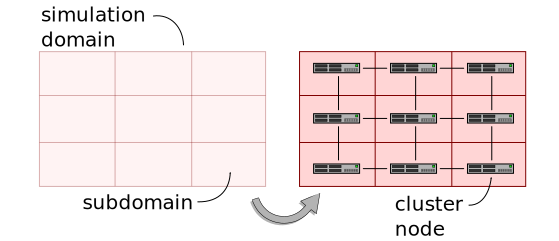
\includegraphics[width=\textwidth]{graphics/30_state_of_the_art}
  \caption{State of the art: the simulation domain is decomposed in
    subdomains. Subdomains are mapped one-to-one onto the homogeneous
    compute cluster.}
  \label{fig:state_of_the_art}
\end{figure}

\todo{Rearrange graphic mentioned by Carli}

For most simulations computed on cluster systems is this approach
state of the art.  This approach works, as long as both hardware and
simulation stay in this fixed relationship. Thus, there is no change
necessary as long as a simulation will always be executed on the same
cluster, with the same network topology and the same algorithms
describing the simulation model.

However, it is not possible to map all modern simulations in this
model of a homogeneous world, some simulation applications have also
vertical and horizontal heterogeneous behavior.  In vertical
direction, multiscale effects, each representing a specific algorithm
of the simulation, lead to varying communication topologies between
subdomains. Every communication topology usually requires
sophisticated programming, that can be quite time consuming.  In
horizontal direction, the workload of subdomains vary throughout the
time of simulation. Therefore, sooner or later the simulation runs
into an unbalanced state of workload distribution. That unbalanced
state do neither saturates all available compute resources nor does it
reduce overall simulation time to its minimum. Furthermore, a globally
increased workload might require a redistribution of the simulation
domain onto the computing nodes.

Not only the simulation can be heterogeneous, but also the cluster
hardware on which the simulation is executed
(Section~\ref{sec:accel}): vertical cluster heterogeneity is the
development of cluster nodes to multisocket, multicore and
additional accelerator hardware, where each of this compute devices
has its own hierarchical memory structure. This hardware needs to be
programmed with caution and knowledge about the device to achieve
maximal performance.  Also, horizontal differences of cluster nodes
are possible. For example, a cluster can consist of varying node
types for different tasks in the simulation application. Therefore,
the simulation domain can not be mapped one-to-one on such a cluster
configuration, but rather the mapping should be configurable
explicitly. Figure~\ref{fig:heterogeneous_cluster_node} shows such
an explicit mapping from the simulation domain onto a heterogeneous
compute system. This example computing systems shows several device
hierarchies. A single node has two sockets each equipped with a
multicore CPU and each CPU has access to a pair of accelerator
devices.

\begin{figure}[H]
  \centering
  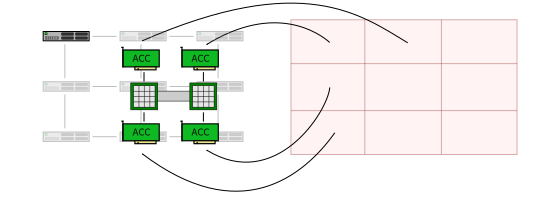
\includegraphics[width=\textwidth]{graphics/30_heterogeneous_cluster_node}
  \caption{Explicit mapping of subdomains onto the computing nodes}
  \label{fig:heterogeneous_cluster_node}
\end{figure}

A real world example for such heterogeneous behavior of simulations is
the PIConGPU simulation (Section \ref{sec:picongpu}). While magnetic
and electric fields only influence their directly neighboring fields,
which requires next neighbor communication, particles interact
globally with each other, which requires an all to all communication
algorithm.  Furthermore, during the time of the simulation, particles
can move to other subdomains, which leads to an unbalanced
distribution of particles over the entire simulation domain. On the
hardware side, PIConGPU is developed for the execution on cluster
systems with NVIDIA accelerator hardware.  CPUs are responsible for
data offloading and communication over the network, some of the
available accelerators compute the interaction of fields and
particles, while others generate a visualization of the simulated
data. Thus, vertical and horizontal heterogeneity both in simulation
domains and on hardware cluster are already present in real world
simulation applications.

Nowadays, state of the art communication libraries can not be adapted
to the needs of modern simulation applications.  Therefore, there
should be an interlayer between simulation application and the
software stack of the cluster. This layer should allow for an explicit
mapping of the simulation domain onto the communication library, while
the communication library should be easily exchangeable. With such a
setup, the mapping can be adjusted to heterogeneous behavior of
simulation application and cluster hardware.  As an added benefit,
this layer can be used to address problems like load balancing and
fault tolerance. However, both of these problems will not be addressed
by this system directly. Instead it should be possible to build an
application that supports both fault tolerance and load balancing
based on this system.

To address these issues, an approach for a flexible mapping of
communication processes onto arbitrary communication libraries was
designed This design will be presented in the following
sections. First of all, the requirements for such a system are
discussed. It is followed by a description of the overall design and
finally the design of each component is discussed in detail.


%%%%%%%%%%%%%%%%%%%%%%%%%%%%%%%%%%%%%%%%%%%%%%%%%%%%%%%%%%%%%%%%%%%%%%%%%%%%%%%%
%                                                                              %
% REQUIREMENTS                                                                 %
%                                                                              %
%%%%%%%%%%%%%%%%%%%%%%%%%%%%%%%%%%%%%%%%%%%%%%%%%%%%%%%%%%%%%%%%%%%%%%%%%%%%%%%%
% Checked
\subsection{Requirements}
\label{sec:requirements}

The previous section described the state of the art of simulations on
cluster systems and gave a motivation to solve the problems of modern
simulations. It was claimed that an interlayer between application and
communication library is required.  This interlayer should offer the
possibility to describe the communication processes of the simulation
in a very general manner.  The construction of this interlayer
involves three steps.  First of all, existing communication libraries
should be abstracted by a general communication interface. Thus,
communication is not restrict to a single communication library and,
therefore, makes the simulation more portable.  Furthermore, The
communication topology of the simulation should be modeled explicitly.
So that, the modeled communication topology can be mapped explicitly
onto an communication abstraction.  Finally the combination of modeled
communication topology and the abstraction from communication
libraries form an approach to communicate virtually on basis of the
described communication topology.  In summary, the discussion on the
interlayer result in the following four requirements of the referred
problems of modern simulations:

\begin{enumerate}
\item Abstract data exchange method
\item Description of the communication topology
\item Mapping of communiation topology onto the abstract topology
\item Virtual data exchange method 
\end{enumerate}


%%%%%%%%%%%%%%%%%%%%%%%%%%%%%%%%%%%%%%%%%%%%%%%%%%%%%%%%%%%%%%%%%%%%%%%%%%%%%%%%
%                                                                              %
% ANALYSIS OF PIConGPU CODE                                                    %
%                                                                              %
%%%%%%%%%%%%%%%%%%%%%%%%%%%%%%%%%%%%%%%%%%%%%%%%%%%%%%%%%%%%%%%%%%%%%%%%%%%%%%%%
\section{Analysis of PIConGPU-Code}
\label{sec:picongpu_analysis}

\todo{Entscheiden ob das fliegt oder noch drin bleibt}

The analysis of the PIConGPU source code and modeled simulation domain
plays as significant role in the design of the developed system.

\begin{itemize}
\item How does the communication topology look like?
  \begin{itemize}
  \item Domain is divided into a 3-dimensional grid of cells
  \item Two different types of effects : particles and fields
  \item Fields do next neighbor communication 
  \item Particles need all-to-all communication
  \end{itemize}

  \item What kind of communcation layer is used?
    \begin{itemize}
      \item Communication is based on MPI and CUDA memcpy
      \item MPI used for communication over subdomain borders (p2p and collective)
      \item CUDA memcpy used for offload of simulation data from 
        host cpu to accelerator device and vice versa
    \end{itemize}

  \item How is Communication implemented in PIConGPU ?
    \begin{itemize}
      \item Simulation data is stored in gridbuffer
      \item Gridbuffer does automatically offload to accelerator
      \item Gridbuffer knows its neighbor gridbuffers which
        are calculated by a function
      \item Communication operations are handled by a communicator class
      \item Collective operations are directly implemented by
        MPI collectives
    \end{itemize}

\end{itemize}


%%%%%%%%%%%%%%%%%%%%%%%%%%%%%%%%%%%%%%%%%%%%%%%%%%%%%%%%%%%%%%%%%%%%%%%%%%%%%%%%
%                                                                              %
% THE SYSTEM                                                                   %
%                                                                              %
%%%%%%%%%%%%%%%%%%%%%%%%%%%%%%%%%%%%%%%%%%%%%%%%%%%%%%%%%%%%%%%%%%%%%%%%%%%%%%%%
% Checked 
\section{Design of the System}

Physical networks such as Ethernet, Infiniband or Myrinet are the
foundation of communication libraries such as MPI
(Section~\ref{sec:MPI}).  State of the art simulation applications are
usually implemented directly on these existing communication
libraries. The developed system introduces an interlayer between
application and communication library (Figure \ref{fig:design}). This
layer fulfills all requirements set up in
Section~\ref{sec:requirements}. Figure \ref{fig:design} shows the
individual components of the interlayer and which requirement they
fulfill. The communication abstraction layer, on top of the existing
communication library, abstracts the communication interface.  A graph
is used to model the communication topology of the simulation domain
and a graph-based virtual overlay network maps this graph onto the
hardware topology of the communication abstraction layer.

\begin{figure}[H]
  \centering 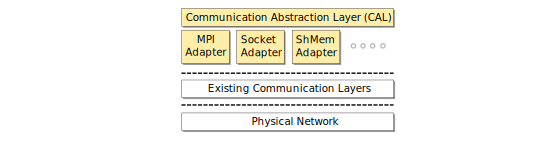
\includegraphics[width=\textwidth]{graphics/30_design}
  \caption{Design of the developed system in layers. An intermediate
  layer between application and communication library is introduced.}
  \label{fig:design}
\end{figure}

\todo{replace description by modeling}

This section presents the design of the system that fulfills the
previously discussed requirements (Section~\ref{sec:requirements}).
It will discuss each component in detail, starting with the
communication abstraction layer in
Section~\ref{sec:comm_abstraction}. Then, the graph interface is
described in Section~\ref{sec:graph}, finally, the graph-based virtual
overlay network is introduced in Section~\ref{sec:gvon}. Component
interfaces will be described in some cases by pseudo-code which is
strongly related to the C++ programming language. It is assumed, that
the reader has a basic knowledge of programming and function
interfaces.

\todo{Reference of pseudo code}

%%%%%%%%%%%%%%%%%%%%%%%%%%%%%%%%%%%%%%%%%%%%%%%%%%%%%%%%%%%%%%%%%%%%%%%%%%%%%%%%
%                                                                              %
% COMMUNICATION ABSTRACTION LAYER                                              %
%                                                                              %
%%%%%%%%%%%%%%%%%%%%%%%%%%%%%%%%%%%%%%%%%%%%%%%%%%%%%%%%%%%%%%%%%%%%%%%%%%%%%%%%
% Checked
\section{Abstraction from Existing Communication Layers}
\label{sec:comm_abstraction}

% Motivation for communication abstraction
Simulation applications can be interconnected by a vast variety of
communication libraries. Most simulations use exactly one possible
libarary, but this restricts the simulation to compute systems which
support only the selected library (Figure
\ref{fig:design_state_of_the_art}).

\begin{figure}[H]
  \centering \includegraphics[width=\textwidth]{graphics/30_design_state_of_the_art}
  \caption{State of the art: simulation applications are implemented directly
  on top of the communication library.}
  \label{fig:design_state_of_the_art}
\end{figure}

\todo{Replace Existing communication layer by existing communication libraries}

Assuming that a simulation, distributed on a several computers, uses a
communication library based on TCP/IP sockets. The execution of this
simulation on a single machine is an interesting use case for
testing. It results in no problem when the simulation is executed on
this local machine and communicates locally by sockets.  But, it might
be more efficient to use shared memory to exchange data between
subdomains, instead of TCP/IP messages.

\todo{Reference that shared memory is faster than TCP/IP}

However, replacing one interface for data exchange by another is not
the solution of the problem, since, this usually requires a lot of
reprogramming of the communication logic.  Rather, varying
communication libraries should by addressable by the same
communication interface to make the application portable for varying
computing environments. Although, there are existing standards for
communication in cluster systems, the world of computer science is
subject to constant change.  The possibility to exchange the
underlying layer without changing the interface to this layer is a
precondition for future applications in distributed computing.  Thus,
the abstraction from this existing communication libraries is a
fundamental property for a portable application.

The challenge is to provide a very general interface, that provides
the possibility to address varying communication libraries through it.
This interface should be as common as possible and should be easily
deployable into existing applications by replacing the actual
communication library without changing the fundamental understanding
of the way to communicate within this application. The following
section describes the design of such an abstract communication
interface.


%%%%%%%%%%%%%%%%%%%%%%%%%%%%%%%%%%%%%%%%%%%%%%%%%%%%%%%%%%%%%%%%%%%%%%%%%%%%%%%%
%                                                                              %
% CAL                                                                          %
%                                                                              %
%%%%%%%%%%%%%%%%%%%%%%%%%%%%%%%%%%%%%%%%%%%%%%%%%%%%%%%%%%%%%%%%%%%%%%%%%%%%%%%%
% Checked
\subsection{Communication Abstraction Layer (CAL)}
\label{sec:cal}

The \textit{Communication Abstraction Layer}, short \textit{CAL}, is a
general communication interface on top of an existing communication
library. The libraries are accessible through adapters, which makes it
possible to access varying communication libraries. By exchanging the
adapter, the application based on the interface can be ported to
varying communication libraries without changing interface function
calls. The CAL is configured with a certain adapter at compile
time. Thus, by using this flexible approach, no run-time overhead
should occur.

While the CAL provides an abstract interface with common communication
methods, the adapter implements the interface demanded by the CAL.
Particular communication operations are performed by existing
communication libraries encapsulated in the adapter.

Instances participating on communication in general are subsequently
called peers.
\todo{Could be a footnote}
The interface of the CAL provides basic point-to-point
communication operations, collective operations
(Section~\ref{sec:cal_comm}) and operations for grouping of peers
(Section~\ref{sec:cal_context}).  Figure \ref{fig:cal} shows
the communication abstraction layer on top of existing communication
libraries.  The CAL with a specific adapter could already replace a
specific communication library in simulation applications, but it
is not meant to be the level of abstraction the simulation programmer
will interact with. Further layers of abstraction will be discussed in
Sections \ref{sec:graph} and \ref{sec:gvon}.

\begin{figure}[H]
  \centering
  \includegraphics[width=\textwidth]{graphics/30_design_cal}
  \caption{Communication Abstraction Layer (CAL) on top of existing
    communication layers. Varying communication libraries can be
    addressed through the CAL interface, when an according adapter for
    this library is implemented.}
  \label{fig:cal}
\end{figure}

\todo{physical network to far from line}

Using the CAL instead of a concrete communication library has
the advantage, that only the adapter needs to be replaced when
changing the communication environment, for example when migrating
to another compute architecture. Although, the application has
to be recompiled, the CAL interface stays the same.


%The CAL has the requirement, that peers need to be connected directly
%by the network of the adapter.
%Peers have to be connected directly by the network of the
%adapter.
%Because, It is not planed that the CAL provides routing
%abilities.
%No routing makes it impossible to forward data between
%different adapters of the CAL. Thus a specific CAL only provides a
%single adapter.
%But several CALs can be used with different adapters
%to communicate on several networks.
%In such a scenario a kind of
%routing can be implemented on top of the CAL by the system
%user.
%Therefore, the design was first pushed forward in the direction
%of a single adapter design and considerations regard to a multiple
%adapter design is left open for future work.


%%%%%%%%%%%%%%%%%%%%%%%%%%%%%%%%%%%%%%%%%%%%%%%%%%%%%%%%%%%%%%%%%%%%%%%%%%%%%%%%
%                                                                              %
% ADDRESSING OF PEERS                                                          %
%                                                                              %
%%%%%%%%%%%%%%%%%%%%%%%%%%%%%%%%%%%%%%%%%%%%%%%%%%%%%%%%%%%%%%%%%%%%%%%%%%%%%%%%
% Checked
\subsection{Addressing of Peers}
% CAL virtual addressing
Each communication library comes with its own way to address peers,
which can be quiet different. Internet socket based systems address
their peers by IP addresses, MPI based systems address their processes
by ranks and systems based on shared memory are using memory
addresses.  These diverse approaches to address peers in a network
need to be translated to an unified address space to provide a
singular interface for the CAL user.  Therefore, the CAL provides a
virtual address which is an unique identifier for its peer. The
virtual address will sometimes be abbreviated by \emph{vAddr}.
\todo{could be footnote} Based on this virtual address, peers are able
to address each other through the CAL interface.

The translation of virtual addresses to the adapter specific real
address is resolved by the adapter itself. Thus, the adapter defines
how the participants of its network are mapped onto the given virtual
address space of the CAL. This mapping is hidden from the CAL, so that
the CAL only needs to handle virtual addresses and the adapter handles
its particular address space.

%%%%%%%%%%%%%%%%%%%%%%%%%%%%%%%%%%%%%%%%%%%%%%%%%%%%%%%%%%%%%%%%%%%%%%%%%%%%%%%%
%                                                                              %
% CAL INTERFACE                                                                %
%                                                                              %
%%%%%%%%%%%%%%%%%%%%%%%%%%%%%%%%%%%%%%%%%%%%%%%%%%%%%%%%%%%%%%%%%%%%%%%%%%%%%%%%
\subsection{Communication Interface}
\label{sec:cal_comm}
% Peer2Peer Operations
\subsubsection*{Point-to-Point Communication Methods}

In the first place, the CAL provides point-to-point communication. This is composed of
basic communication methods to exchange abitrary data between two
peers, such as sending and receiving.  These operations are available
blocking and non-blocking variants.

A Non-blocking communication method returns an event object that represents
the state of the only just executed communication method. The state
of the event is either \emph{ready} or \emph{not ready}. An
event provides a function to request the current state and a function
to  wait until the method has finished. The CAL only provides the
the event interface, adapters implement the CAL interface for their
particular communication library since each libary treats non-blocking
communication differently \cite{ref:mpi_specification,ref:boost_asio}.

A point-to-point communication operation is called with a triplet of
arguments, including the virtual address of sender or receiver, the
message description tag and the actual data object to exchange.  The
interface is influenced by existing communication libraries that all
share a common interface \cite{ref:boost_mpi, ref:boost_asio,
  ref:zmq}. The message description tag is a simple header of the
message. It helps to easily distinguish between messages of the same
sending peer.  The data object should provide methods to retrieve the
data pointer and the size of the data. The data pointer should point
to a contiguous memory area. The following list shows the
point-to-point communication operations of the CAL interface:

\begin{itemize}
  \item  \textbf{void send(destination vaddr, tag, data)}
  \item  \textbf{void recv(source vaddr, tag, data)}
  \item  \textbf{Event asyncSend(destination vaddr, tag, data)}
  \item  \textbf{Event asyncSecv(source vaddr, tag, data)}
\end{itemize}

%%%%%%%%%%%%%%%%%%%%%%%%%%%%%%%%%%%%%%%%%%%%%%%%%%%%%%%%%%%%%%%%%%%%%%%%%%%%%%%%
%                                                                              %
% CONTEXT                                                                      %
%                                                                              %
%%%%%%%%%%%%%%%%%%%%%%%%%%%%%%%%%%%%%%%%%%%%%%%%%%%%%%%%%%%%%%%%%%%%%%%%%%%%%%%%
% Checked
\subsubsection*{Grouping of peers}
\label{sec:cal_context}
Grouping of peers is, next to the communication methods, the most
important function the CAL provides through its interface.  By
default, all peers of the CAL are grouped to a global group of peers.
A group of peers will be called \textit{context}. Therefore, the
global group of peers is called global context. A context is valid for
all contained peers. In turn, it is invalid for all peers not
contained.

A context stores the information about the virtual addresses of the peers , the
number of peers grouped and whether the context is valid for a particular
peer. It is the base for communication algorithms with more than 2
participating peers.
% These algorithm are introduced as collective operations (Section \ref{sec:cal_collective}).

The CAL provides always the global context from which a peer can
retrieve its global virtual address. A new context can be created from
a subset of peers of an already existing context. Thus, a new context
can be created according to the requirements of the communication
algorithm. This new context provides its own virtual address space,
thus, the virtual address of a peer is context dependent.

Managing of contexts is specific for the chosen adapter. The CAL only
defines the context interface, but each adapter needs to implement a
context for its particular communication library. Furthermore, the
adapter must respect that a virtual address is context
dependent. Therefore, the mapping of a virtual address to a real
address has to be adapted to the currently used context.

%%%%%%%%%%%%%%%%%%%%%%%%%%%%%%%%%%%%%%%%%%%%%%%%%%%%%%%%%%%%%%%%%%%%%%%%%%%%%%%%
%                                                                              %
% COLLECTIVE OPERATIONS                                                        %
%                                                                              %
%%%%%%%%%%%%%%%%%%%%%%%%%%%%%%%%%%%%%%%%%%%%%%%%%%%%%%%%%%%%%%%%%%%%%%%%%%%%%%%%
% Checked
\subsubsection*{Collective Operations}
\label{sec:cal_collective}
A \textit{collective operation}, short \textit{collective}, is a
communication pattern that is executed simultaneously by all peers of
a context. For example are collectives used to collect, distribute,
share and reduce data.  Each collective can be implemented by a
sequence of peer to peer operations, but communication libraries,
especially the ones for high performance calculations, often come with
optimized collective support \cite{ref:mpi}.

A collective is always executed with respect to a context and the
result is either received by only one peer, the root, or by all peers.
While a large number of collectives is known to the parallel
computation commmunity, the CAL only provides the most common ones
with respect to the analysis of the PIConGPU source code
(Section~\ref{sec:picongpu_analysis}).  \todo{Footnote that other
  collectives are easily deploy able in future work} The following is
a list of all provided collective operations of the CAL and their
description:


\begin{itemize}
\item  \textbf{gather(root vAddr, context, send, recv)}\\
  Collection of data elements from every peer in the context. Each peer
  contributes the same number of data elements. The collected data will
  be received from the root peer.

\item \textbf{allGather(context, send, recv)}\\
  Similar to gather(), but all peers of the context receive the data.

\item  \textbf{scatter(root vAddr, context, send, recv)}\\
  Distribution of data elements from the root peer to all other peers of
  the context. The data will be divided into chunks of same
  size. Assuming the number of data elements is divisible by the number
  of peers, every peer will receive the same number of data
  elements. Thus, every peer receives different data elements.

\item  \textbf{allScatter(context, send, recv)}\\
  Similar to scatter(), but all peers of the context receive the same.

\item  \textbf{reduce(root, context, operation, send, recv)}\\
  Reduction of the data elements from every peer of a context
  by a binary function that takes arguments of an arbitrary type
  and returns a values of the same type.

\item  \textbf{allReduce(context, operation, send, recv)}\\
  Similar to reduce(), but all peers of the context receive the
  result of the reduction.

\item  \textbf{void broadcast(root, context, data)}\\
  Distributes data elements from the root peer to all other peers of
  the context. Every peer receives the same data elements.

\item  \textbf{syncronize(context)}\\
  This operation synchronizes the control flow of all peers of the
  context.

\item  \textbf{createContext(peers, context)}\\ 
  Creation of a new context from a subset of peers of an already
  present context.

\end{itemize}

The listed collectives have all homogeneous behavior. All peers either
send or receive the same number of elements.  Some algorithms require
an exchange of varying number of data elements. Thus, collectives like
gather, allGather, scatter, allScatter are also available in a variant
with varying number of data elements per peer. These collectives get
an additional receive count argument, that describes how many data
elements each peer has contributed to the collective.


%%%%%%%%%%%%%%%%%%%%%%%%%%%%%%%%%%%%%%%%%%%%%%%%%%%%%%%%%%%%%%%%%%%%%%%%%%%%%%%%
%                                                                              %
% GRAPH                                                                        %
%                                                                              %
%%%%%%%%%%%%%%%%%%%%%%%%%%%%%%%%%%%%%%%%%%%%%%%%%%%%%%%%%%%%%%%%%%%%%%%%%%%%%%%%
\section{Modeling of the Application Domain by a Graph}
\label{sec:graph}
A simulation application always implements a particular algorithm
that describes a particular model.

This Algorithm often requires a
domain decomposition (Section \ref{sec:domain_decomposition}) of the
simulation domain into a set of subdomains. Assume, subdomains need
to interact with each other, communication between subdomains is
necessary. Thus, the algorithm of the simulation determines
the communication topology.



%The simulation domain is mapped fixed onto the compute resources.
This communication topology is often implemented in a implicit and
static manner.  Because the communication topology is not modeled
explicit, a change of the simulation algorithm needs to be translated
into a change of the corresponding communication patterns, which can
be quiet costly.

\paragraph*{}
A more elegant approach is to explicitly model the relationships
between the subdomains and therefore the communication topology. The
most general method to model a topology is a \textit{graph}
\cite{ref:graph}.  From a mathematical perspective, a graph is a pair
of vertices and edges. Edges are pairs of vertices. So to speak, a
graph represents a set of objects, where some of these objects are
connected by links.

Changing the simulation domain implies a different communication
topology and in turn implies a different graph.  Since, the
communication topology is explicit modeled by a graph, it is not
necessary to rewrite the simulation application as long the
application is oriented on the topology information provided by the
graph. Thus, algorithms can by implemented on top of the graph
description.

% directed cycle multi graph
The graph has the property, that vertices are connected by directed edges. Loops
and multiple edges between two vertices are allowed (Figure
\ref{fig:graph}). The resulting graph is a directed multi graph with
loops. The mathematical expression for this kind of graph is quiver
\cite{ref:quiver}

\begin{figure}[H]
  \centering 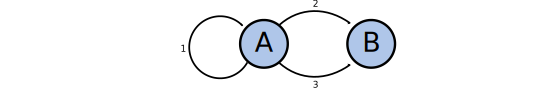
\includegraphics[width=\textwidth]{graphics/30_graph}
  \caption{The graph interface describes quivers. It is shown a directed cycle multi graph with four vertices.}
  \label{fig:graph}
\end{figure}

The presented graph should be addressable by the following interface:

\begin{itemize}
  \item \textbf{getVertices}()\\
    Returns the list of all vertices of the graph.
    
  \item  \textbf{getVertex(index)}\\
    Returns a particular vertex by vertex index.

  \item  \textbf{getAdjacentVertices(vertex)}\\
    Returns a list of all adjacent vertices of vertex.

  \item  \textbf{getOutEdges(vertex)}\\
    Returns a list of all outgoing edges from the vertex
    paired with their target vertex.

  \item  \textbf{getInEdges(vertex)}\\
    Return a list of all incoming edges to the vertex 
    paired with their source vertex.

  \item  \textbf{createSubGraph(vertices)}\\
    Returns a subgraph, that only contains the defined
    vertices from the supergraph.
\end{itemize}

%%%%%%%%%%%%%%%%%%%%%%%%%%%%%%%%%%%%%%%%%%%%%%%%%%%%%%%%%%%%%%%%%%%%%%%%%%%%%%%%
%                                                                              %
% GRAPH PROPERTIES                                                             %
%                                                                              %
%%%%%%%%%%%%%%%%%%%%%%%%%%%%%%%%%%%%%%%%%%%%%%%%%%%%%%%%%%%%%%%%%%%%%%%%%%%%%%%%
\subsection{Properties}
A graph alone is just the representation of connected vertices, but
has no connection to the simulation domain. The connection usually
only exists in the head of the programmer of the simulation
application. But, a graph can be interpreted as a container, wherby the
objects of the container are in a relation to each other.

The container object will be called property and is introduced as a
concept to annotate a graph. A property provides subdomain information
and can be bound to vertices and edges (Figure
\ref{fig:property}). Vertices and Edges of the same graph share
respecively the same type of property. A graph annoted with properties
is significantly more meaningful and thus helps to keep the connection
of the simulation domain and communication topology.

\begin{figure}[H]
  \centering 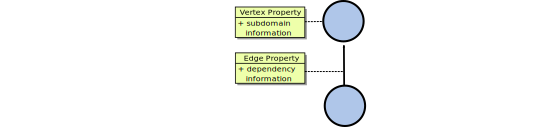
\includegraphics[width=\textwidth]{graphics/30_property}
  \caption{A graph with both vertex and edge properties. The vertex
    property primarily describe a subdomain. The edge property
    describe the dependencies between subdomains.}
  \label{fig:property}
\end{figure}

A Property can also be used to create a connection between a pair of
graphs. Thus a modeling of hiararchical domains is also possible.  A
later example will make use of this hierarchical modeling (Section
\ref{sec:gol}).

%%%%%%%%%%%%%%%%%%%%%%%%%%%%%%%%%%%%%%%%%%%%%%%%%%%%%%%%%%%%%%%%%%%%%%%%%%%%%%%%
%                                                                              %
% MODELING GAME OF LIFE AS A GRAPH                                             %
%                                                                              %
%%%%%%%%%%%%%%%%%%%%%%%%%%%%%%%%%%%%%%%%%%%%%%%%%%%%%%%%%%%%%%%%%%%%%%%%%%%%%%%%
\subsection{Modeling Game of Life as a Graph}
\label{sec:gol}
To give an example for modeling a specific simulation application,
Figure \ref{fig:gol_modeling} shows the modeling of the Game of Life (GoL) \cite{ref:gol}
domain by a graph. GoL simulates the state evolution of a set of cells for
an abitrary amount of time steps. The cells are arranged in a two-
dimensional grid (Figure \ref{fig:gol_simulation}).  A cell has a
state which is either alive or not alive and the state of the next
time step is calculated by rules. The common set of rules determine
the state of a cell for the next time step by the state information of
the neighboring cells. One rule is, that a dead cell with
exactly 3 living cells in the neighborhood will be reborn on the next
time step. For the further description of GoL it is assumed that only
this rule exists.

\begin{figure}[H]
  \centering 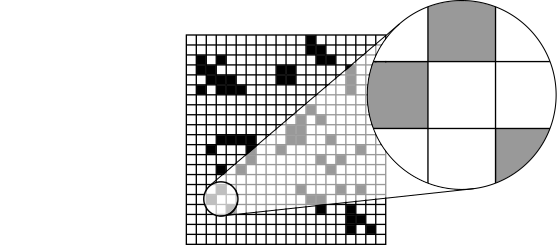
\includegraphics[width=\textwidth]{graphics/30_gol_simulation}
  \caption{A GoL domain with a cut out of 9 neighboring cells. Cells have
  a state, while living cells are colored dark, dead cells are white.}
  \label{fig:gol_simulation}
\end{figure}

Modeling this common rule straight forward, ending up in a graph where
every cell of the GoL world is represented by a vertex and neighboring
cells are connected by an edge. Each vertex has the property cell, that
contains the state of the cell. Figure \ref{fig:gol_modeling} shows a vizualized
cut out of the GoL modeled domain. To determine the next state of a 
cell, it has to count the living adjacent cells in the graph and if
exactly three adjacent cells are alive, then the cell will also be
alive on the next time step.

\begin{figure}[H]
  \centering 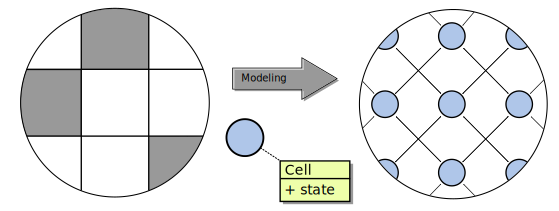
\includegraphics[width=\textwidth]{graphics/30_gol_modeling}
  \caption{Cut-out of a Game of Life domain (on the left) was modeled
    as a graph (on the right). Each Vertex is described by the vertex
    property cell, containing the state information of the cell. A
    Vertex determines next state by state of neighboring cells}
  \label{fig:gol_modeling}
\end{figure}

Changing this rules slightly to a GoL where a cells as alive in the
next time step when at least one diagonal neighbor is alive.  Thus,
this changes the GoL communication topology and therefore the
graph. Figure~\ref{fig:gol_modeling_changed} models the GoL domain
with the changed rule. Vertices are connected with its diagonal
located vertices. Nonetheless, to determine the next state of a cell,
it has to count the living cells of of connected cells in the graph.

\begin{figure}[H]
  \centering \includegraphics[width=\textwidth]{graphics/30_gol_modeling_changed}
  \caption{Cut-out of a Game of Life domain (on the left) modeled
    with a different rule. Only diagonal located vertices are connected.}
  \label{fig:gol_modeling_changed}
\end{figure}


%%%%%%%%%%%%%%%%%%%%%%%%%%%%%%%%%%%%%%%%%%%%%%%%%%%%%%%%%%%%%%%%%%%%%%%%%%%%%%%%
%                                                                              %
% PARTITIONING THE GoL GRAPH                                                   %
%                                                                              %
%%%%%%%%%%%%%%%%%%%%%%%%%%%%%%%%%%%%%%%%%%%%%%%%%%%%%%%%%%%%%%%%%%%%%%%%%%%%%%%%
\subsection{Partitioning the GoL Graph}
The graph in figure \ref{fig:gol_modeling} models the GoL domain very fine
granular by every individual cell. While it is the smallest possible
domain decomposition, it might not be very efficient when this graph
is the foundation for a distributed computing application. Imagining, a
single cell is calculated by a process and the cell state is exchanged
by inter-process communication, but single process can compute
considerably more cells.

Figure \ref{fig:gol_bundle} shows the partioning of the fine granular
GoL graph by bundling multiple vertices together to a partioned
graph. A parition of vertices is called a bundle. These Bundles are
connected by edges when at least one cell on the border of a bundle
is the neighbor of a border cell from another bundle.  The creation of
a partioned graph by bundles with a minimum of connections is the
topic graph partitioning algorithms. But the modeling of an optimal
partitioned graph is not part of this work.

While the fine granular GoL graph represents the GoL cells in detail, the
partitioned graph represents dependencies of bundled cells. Thus
the properties of the partioned graph changed such that bundles
have store the cells they bundle and edges refer to neighboring
cells.

\begin{figure}[H]
  \centering 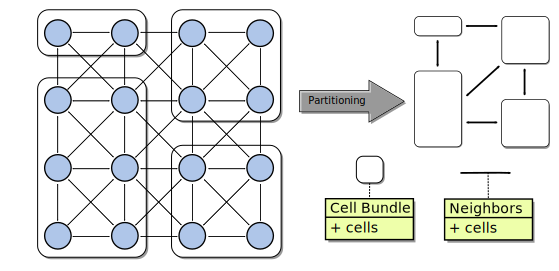
\includegraphics[width=\textwidth]{graphics/30_gol_bundle}
  \caption{The GoL graph is partitioned by bundling multiple
    cells. The properties of the partioned graph have changed, such
    that the vertex property contains the cells of a bundle, while the
    edge property contains information about neighboring cells.}
  \label{fig:gol_bundle}
\end{figure}

The partitioned graph could be used as foundation to distribute GoL to
multiple devices on a cluster. Each bundle could be computed by an own
process. The Processes do calculation for their local GoL graph and
communicate states of their border cells to adjacent bundles.

It has been shown a different approach to model the Game of Life
domain. It were used the same description language; the graph.
Fine granular modeled domains can be partioned by common graph
partition algorithm to obtain possibly more performance by
clustering vertices.


%%%%%%%%%%%%%%%%%%%%%%%%%%%%%%%%%%%%%%%%%%%%%%%%%%%%%%%%%%%%%%%%%%%%%%%%%%%%%%%%
%                                                                              %
% MODELING GAME OF LIFE AS A GRAPH                                             %
%                                                                              %
%%%%%%%%%%%%%%%%%%%%%%%%%%%%%%%%%%%%%%%%%%%%%%%%%%%%%%%%%%%%%%%%%%%%%%%%%%%%%%%%
\subsection{Modeling a N-Body Simulation as Graph}
\ref{sec:design:nbody}
An N-body simulation is a simulation of particles influenced by
physical forces. The force considered for this simulation is the
gravity among each particle in the domain.  A particle is described by
mass $m$, location $\overrightarrow{r}$ and velocity $\overrightarrow{v}$.  The gravitational forces
between two particles $i$ and $j$ can be calculated in a two-body model 
with the gravitationlal constant $G$ by the equation \ref{eq:two_body_force}:

\begin{equation}
  \label{eq:two_body_force}
  \overrightarrow{F_{i,j}} = G  m_i  m_j \cdot \frac{\overrightarrow{r_j} - \overrightarrow{r_i}}{|\overrightarrow{r_j} - \overrightarrow{r_i}|^3}
\end{equation}

The gravitational force of particle $i$ to all other N-1 particles
is the sum of each particluar force $\overrightarrow{F_{i,j}}$(Equation~\ref{eq:n_body_force}).

\begin{equation}
  \label{eq:n_body_force}
  \overrightarrow{F_{i,n}} = \sum_{j = 0 \atop j \neq i}^{N-1} \overrightarrow{F_{i,j}}
\end{equation}

Thus, to calculate the force affecting particle $i$, mass and
loacation of all other particles have to be considered. Modeling the
dependencies resulting from the simulations algorithm results in an
all to all communcation pattern with a complexity of $o(N^2)$. Figure
\ref{fig:nbody_modeling} models the N-body domain with $N = 6$ as a
fully connected graph. Particles are represented as pentagon in a
two-dimensional space. The size of the particles signals its mass and
the arrow its velocity and move direction.  In the modeling, a vertex
represents a particle and all particles are connected by an edge. A
vertex has the property particle that includes the particle mass,
location and velocity.

\begin{figure}[H]
  \centering 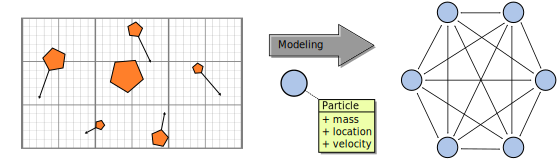
\includegraphics[width=\textwidth]{graphics/30_nbody_modeling}
  \caption{Modeling of an N-body domain with $N = 6$. A particle is represented
  by a vertex and all vertices are connected with each other by an edge.}
  \label{fig:nbody_modeling}
\end{figure}

A force on the particle results in a change of its velocity and a
in a changed location for a fixed amount of time $t$. Calculating
the results of equations \ref{eq:n_body_update} updates these
values of the particle.
\begin{align}
  \label{eq:n_body_update}
  \overrightarrow{a} =&~ \frac{\overrightarrow{F_{i,n}}}{m}\\
  \overrightarrow{v} =&~ \overrightarrow{a} \cdot t + \overrightarrow{v_0}\\
  \overrightarrow{r} =&~ \frac{\overrightarrow{a}}{2} \cdot t^2 + \overrightarrow{v_0} \cdot t + \overrightarrow{r_0}
\end{align}




%%%%%%%%%%%%%%%%%%%%%%%%%%%%%%%%%%%%%%%%%%%%%%%%%%%%%%%%%%%%%%%%%%%%%%%%%%%%%%%%
%                                                                              %
% GRAPH-BASED VIRTUAL OVERLAY NETWORK (GVON)                                   %
%                                                                              %
%%%%%%%%%%%%%%%%%%%%%%%%%%%%%%%%%%%%%%%%%%%%%%%%%%%%%%%%%%%%%%%%%%%%%%%%%%%%%%%%
\section{Graph-Based Virtual Overlay Network (GVON)}
\label{sec:gvon}
The previous sections described the tools to communicate and to model
the communication topology. By providing an explicit mapping of the
communication topology onto the abstract communication layer. The
combination of these tools establish a virtual communication layer
within the simulation domain.  Such that, communication between
subdomains of the application can be represented. Therefore, this
section introduces a \textit{graph-based virtual overlay network},
short \textit{GVON}, that is based on the graphs and the CAL.

The graph does provide a simulation domain specific communication
topology.  It is used as a blueprint for the virtual network topology.
Communication operations are provided by the CAL as base for the
overlay network.  Figure \ref{fig:gvon} shows the GVON as a layer
between the graph and CAL on one side and the application on the other
side.

\begin{figure}[H]
  \centering \includegraphics[width=\textwidth]{graphics/30_gvon}
  \caption{The graph-based virtual overlay network provides
    communication functionality based on the CAL, but uses the
    communication topology modeled by the graph.}
  \label{fig:gvon}
\end{figure}

All peers that want to take part on the communication of the GVON need
to know exactly the same graph. In order to ensure that, the graph can be
constructed in parallel by all peers, loaded from the same file of a
distributed file system or could even be delivered by a master
peer. Furthermore, peers need to use the same adapter configuring its
CAL, otherwise a communication is not possible.


%%%%%%%%%%%%%%%%%%%%%%%%%%%%%%%%%%%%%%%%%%%%%%%%%%%%%%%%%%%%%%%%%%%%%%%%%%%%%%%%
%                                                                              %
% GVON MAPPING                                                                 %
%                                                                              %
%%%%%%%%%%%%%%%%%%%%%%%%%%%%%%%%%%%%%%%%%%%%%%%%%%%%%%%%%%%%%%%%%%%%%%%%%%%%%%%%
\subsection{Mapping of the graph onto the CAL}
\label{sec:mapping}
The connection between a graph and a CAL is a mapping of vertices to
peers, called the vertex map.  A vertex map is valid for a particular
graph. The mapping of vertices to peers is a joint process of all
peers that want participate in the communication based on a particular
graph. This process is divided into two phases

\paragraph*{}
The \textbf{first phase} is the distribution of the vertices of the graph to
the peers (Figure \ref{fig:gvon_mapping}), where every peer gets
assigned a set of vertices. There are a varity of methods to
distribute the vertices.  It could be done totally randomized, round
robin or even dictated by some master peer. The distribution behavior
is defined by the user of the developed system and might be object for
further optimization, but it was not topic of this work to find optimal
distributions.

\begin{figure}[H]
  \centering 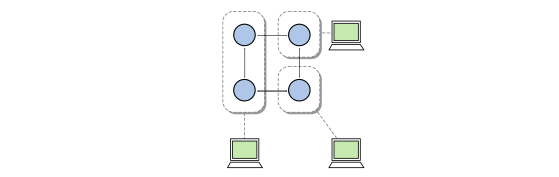
\includegraphics[width=\textwidth]{graphics/30_gvon_mapping}
  \caption{All vertices of a graph are distributed onto 3 peers. The vertices
  are not distributed evenly, thus one peer is host for 2 vertices.}
  \label{fig:gvon_mapping}
\end{figure}

\paragraph*{}
In the \textbf{second phase}, the peers announce their vertices to all other
peers.  A peer that announces vertices is called host and the
announced vertices are called hosted vertices.  Every host receives
from every other host a list of its hosted vertices and stores this
information in its vertex map. A host is responsible for the
communication of its hosted vertices. A host is responsible either for
zero, one or more vertices. So to speak, it is also possible that host
is responsible for all vertices of a graph and communicates finally
always with itself.  Depending on the used adapter this might not even
be a problem, since communication of a peer with itself can be mapped
to local memory copies and does not necessarily go over the network.

Furthermore the GVON provides a mapping of the graph of the announced
vertices to a context (Section \ref{sec:cal_context}), called the
graph map. This mapping is necessary since the GVON will also be used
to map collective operations on the graphs onto the CAL.

The vertex and graph map is the basis for the mapping of communication
processes onto the hardware.


%%%%%%%%%%%%%%%%%%%%%%%%%%%%%%%%%%%%%%%%%%%%%%%%%%%%%%%%%%%%%%%%%%%%%%%%%%%%%%%%
%                                                                              %
% GVON COMMUNICATION                                                           %
%                                                                              %
%%%%%%%%%%%%%%%%%%%%%%%%%%%%%%%%%%%%%%%%%%%%%%%%%%%%%%%%%%%%%%%%%%%%%%%%%%%%%%%%
\subsection{Communication within the GVON}
In the context of an overlay network, a vertex is interpreted as a
virtual peer, edges between adjacent vertices indicate that the
virtual peers are able to communicate with each other. Thus, the
application on top of the GVON has the transparent view, that it is
really exchanging messages between the vertices and the GVON is taking
care, that the messages are reaching the correct vertex host. Thus, 
this level of abstraction is finally the level the application
interacts with.

The GVON provides similar functionality like the introduced
communication operations in the CAL, but on graph basis. Thus both
peer to peer and collective operations are provided.

% GVON P2P
A peer to peer operations within the GVON involves exchanging data
between adjacent vertices over a particular edge of a particular
graph.  These opeations can be blocking or non block, whereby non
blocking operations return an event known from the CAL.  The GVON
provides the following interface for peer to peer operations:

\begin{itemize}
  \item [] void \textbf{send}(graph, destination vertex, edge, data)
  \item [] void \textbf{recv}(graph, source vertex, edge, data)
  \item [] Event \textbf{asyncSend}(graph, destination vertex, edge, data)
  \item [] Event \textbf{asyncRecv}(graph, source vertex, edge, data)
\end{itemize}

The GVON has the task to resolv both the context of a graph and the
host of the source or the destination vertex. This information are
quieried from the vertex and graph map. When this information is
resolved the programm flow is handed over to the CAL. The Cal is then
responsible for exchange data between the hosts.

% GVON collectives
\subsubsection*{GVON Collectives}
Operations between all vertices of a graph can be performed as
collective operations (Section \ref{sec:cal_collective}). A host needs
to perform the collective operation for all its hosted vertices,
otherwise it blocks the execution of the operation.  Thereby, are
collective operations absolutly transpaent to the application. Yet
again, the result of the collective is received by some root vertex or
by all vertices of the graph.

The collective operation is first executed locally for all hosted
vertices of each host. Then it is further handled by the CAL and
transmitted to the receiver(s). Figure \ref{fig:gvon_collective} shows
a gather operation on the same graph and mapping of figure
\ref{fig:gvon_mapping}. A gather operation collects the data of hosted
vertices of a host first locally and uses then the gather operation
provided by the CAL. A similar approach is used for the reduce
operation, whereby data is either collected or reduced locally to a
single value, depending on the commutativity of the reduce
operation. 

The execution of the collective operation can be done sequentially or in
parallel. Both variants have their specific implementation and usage
problems. While sequential execution could lead to dead lock behavior
when a peer forgets to execute the collective for at least one vertex,
a parallel execution needs to ensure that the GVON is implemented in
a thread sage manner.

\begin{figure}[H]
  \centering \includegraphics[width=\textwidth]{graphics/30_gvon_collective}
  \caption{Gather operation with the GVON. Data is first locally 
    and then globally collected. Finally the collected data
    is transmitted to the root vertex.}
  \label{fig:gvon_collective}
\end{figure}


%%%%%%%%%%%%%%%%%%%%%%%%%%%%%%%%%%%%%%%%%%%%%%%%%%%%%%%%%%%%%%%%%%%%%%%%%%%%%%%%
%                                                                              %
% REMAPPING                                                                    %
%                                                                              %
%%%%%%%%%%%%%%%%%%%%%%%%%%%%%%%%%%%%%%%%%%%%%%%%%%%%%%%%%%%%%%%%%%%%%%%%%%%%%%%%
\subsection{Remapping of Vertices}
\label{sec:remapping}
Since, the communication topology is seperated from the communication
layer, it is possible to change the mapping from vertices to peers at
runtime. This runtime behavior is an interesting fact in respect to
load balancing and fault tolerance. A remapping repeats the phases
discussed in the mapping process of distribution and announcement.
Figure \ref{fig:gvon_remapping} shows the remapping of the mapping
from figure \ref{fig:gvon_mapping}. The vertices of the graph is
distributed to now only two peers, while one peer announced three
vertices and the other announces one vertex. The third peer is no
host of this graph anymore.

\begin{figure}[H]
  \centering 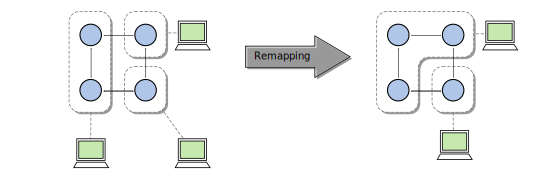
\includegraphics[width=\textwidth]{graphics/30_gvon_remapping}
  \caption{}
  \label{fig:gvon_remapping}
\end{figure}

Load balancing can be an issue when the communication topology is
changing during simulation execution. For example could the GoL
simulation add a new rule, which leads to a changed communication
topology for that in turn exists a better vertex mapping. Even if the
performance of a cluster network link drops, thus, some peers are not
able reach accetable latency and bandwidth between each other, a
remapping could solve this problem at runtime.

A traditional field of application for remapping would be
a moved compute load in the simulation domain. This movement
could be noticed and a remapping could rearrange the compute load
in a fair way.

Another issue is the failure of single cluster nodes and therefore
also a failure of hosts loacted on this nodes. Assuming, that the data
of hosts where backuped, for example through checkpointing techniques,
the hosted vertices of the failed host can be adopted by another host,
also at runtime.

The process of remapping is very similar to the mapping process of
section \ref{sec:mapping}.  It is also divided in two steps:
distribution and announcment. It has to be distinguished between
global and local remapping. A global remapping is a repetition of the
mapping process of section \ref{sec:mapping}. A local remapping does
not require a full redistribution of vertices.  Since the remapping
situation is slightly different, so that host already own a set of
hosted vertices, the distribution is more a swap or occupation of
vertices. 

\cleardoublepage

%%% Local Variables:
%%% TeX-master: "diplom"
%%% End:
